
\section{Erster Abschnitt \initials{M.M.}}
Nach den (Unter-) Kapitelüberschriften soll mit Hilfe von Initialen angegeben werden, wer diesen Abschnitt verfasst hat. Hierzu muss lediglich wie oben im Beispiel gesehen \initials{V.N.} (LaTeX-Code siehe .tex-Datei) hinter einer Kapitelüberschrift eingefügt werden (wobei hier V der Anfangsbuchstabe des Vornamens und N der Anfangsbuchstabe des Nachnamen ist). 
\subsection{Unterabschnitt 1 von Abschnitt 1 \initials{J.M.}}
Eine Aufzählung:
\begin{itemize}
    \item Aufzählungspunkt 1
    \item Aufzählungspunkt 2
	\begin{itemize}
	    \item Aufzählungen können 
	    \item auch verschachtelt werden!
	    \item ...
	\end{itemize}    
    \item Aufzählungspunkt 3
	\begin{enumerate}
	    \item Oder verschachtelt
	    \item \textbf{und} nummeriert!
	    \item ...
	\end{enumerate}
\end{itemize}
Eine andere Art der Aufzählung:
\begin{description}
    \item[Punkt 1: ] Beliebiger Text.
    \item[Punkt 2: ] Beliebiger anderer Text.
\end{description}

\subsection{Unterabschnitt 2 von Abschnitt 1 \initials{M.M.}}
Eine Tabelle:
\par\medskip %Ein mittlerer Absatz
\begin{tabular}{|l|p{4cm}|c|} %1. Spalte linksbündig, 2. Spalte 4cm breit, 3. Spalte zentriert
    \hline
    % Zeile 1:
    Zelle 0,0 & Zelle 0,1 & Zelle 0,2 \\ %Das & trennt die Zelleneinträge voneinander
    \hline
    % Zeile 2:
    Zelle 1,0 & Zelle 1,1 & Zelle 1,2 \\
    \hline
\end{tabular}
\par\smallskip

Mathematische Formel:
\begin{align*} % align zentriert die Formel automatisch
    x &= {\sum}_{i=0}^{n} \frac{y_i}{2} \\ %Durch &= stehen die Gleichheitszeichen untereinander
      &= \pi - 42
\end{align*}
Mathematische Formeln wie $x=x_1 +x_2$ können auch im Fließtext integriert werden. Quellen werden mit \cite{AB12} zitiert und tauchen dann in der Literaturliste auf.

\section{Zweiter Abschnitt \initials{M.M., J.M.}}
Grafiken oder Text können mit multicols nebeneinander arrangiert werden. Mit LaTeX TikZ können auch Graphen oder Automaten modelliert werden:

\begin{multicols}{2} % Multicols ermöglicht es zwei (oder mehr) Grafiken oder Textpassagen nebeneinander anzuordnen. 
Eine Grafik mit TikZ:
	    \begin{figure}[H]
		\centering
		\begin{tikzpicture}[, ->,>=stealth',shorten >=0pt,auto,node distance=3cm,
                semithick, scale=0.9, transform shape]
		\begin{scope}
			\node [state, fill=blue!20] (l0) [label=left:{$\{x\}$}]{$l_0$};
			\node [state, fill=blue!20] (l1) [right of=l0, label=right:{\textcolor{blue}{$10$}}]{$l_1$};
			\node [state, fill=blue!20] (l2) [below of=l0, label=below:{hallo}]{$l_2$};
			
		    	\path (l0) edge [bend left=00] node[xshift=+0.9cm, yshift=-0.46cm] {\parbox{3cm}{$y > 0 /$ \\ $y:=0$}} (l1)
			      (l1) edge [bend left=00] node {$x:=0$} (l2)
			      (l2) edge [bend left=00] node {$x:=y$} (l0);
		\end{scope}
		\end{tikzpicture}
		\caption{Bildunterschrift}
	    \end{figure}
\columnbreak
Eine andere Grafik mit TikZ:
	    \begin{figure}[H]
		\centering
		\begin{tikzpicture}[initial text=, ->,>=stealth',shorten >=0pt,auto,node distance=3cm,
                semithick, scale = 0.9, transform shape]
		\begin{scope}
			\node [state, initial] (r0) {$r_0$};
			\node [state, rectangle] (r1) [right of=r0]{$r_1$};
			\node [state] (r2) [below of=r0] {$r_2$};
			\node [state, accepting] (r3) [below of=r1] {$r_3$};
			
		    	\path (r0) edge [bend left=20] node {$x>10$} (r1)
			      (r1) edge [bend left=20, dashed] node {$x>20/x:=0$} (r0)
			      (r0) edge [dotted] node {\textcolor{red}{fail}} (r2)
			      (r1) edge node {$x\geq15$} (r3)
			      (r2) edge [loop right] (r2);
		\end{scope}
		\end{tikzpicture}
	    \end{figure}
\end{multicols}

Hier kommt nun viel Text. Hier kommt nun viel Text. Hier kommt nun viel Text. Hier kommt nun viel Text. Hier kommt nun viel Text. Hier kommt nun viel Text. Hier kommt nun viel Text. Hier kommt nun viel Text.
\par\smallskip

Hier kommt nun viel Text. Hier kommt nun viel Text. Hier kommt nun viel Text. Hier kommt nun viel Text. Hier kommt nun viel Text. Hier kommt nun viel Text. Hier kommt nun viel Text. Hier kommt nun viel Text. Hier kommt nun viel Text. Hier kommt nun viel Text.
\begin{wrapfigure}[12]{r}{4.5cm} %#1: Zeilenanzahl
    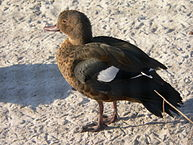
\includegraphics[width=4.3cm]{images/Ente}
    \caption{\small{Quelle: wikimedia}}
\end{wrapfigure}
Hier kommt nun viel Text. Hier kommt nun viel Text. Hier kommt nun viel Text. Hier kommt nun viel Text. Hier kommt nun viel Text. Hier kommt nun viel Text. Hier kommt nun viel Text. Hier kommt nun viel Text. Hier kommt nun viel Text. Hier kommt nun viel Text.  Hier kommt nun viel Text. Hier kommt nun viel Text. Hier kommt nun viel Text. Hier kommt nun viel Text. Hier kommt nun viel Text. Hier kommt nun viel Text. Hier kommt nun viel Text. Hier kommt nun viel Text. Hier kommt nun viel Text. Hier kommt nun viel Text. Hier kommt nun viel Text. Hier kommt nun viel Text. Hier kommt nun viel Text. Hier kommt nun viel Text. Hier kommt nun viel Text. Hier kommt nun viel Text. Hier kommt nun viel Text. Hier kommt nun viel Text. Hier kommt nun viel Text. Hier kommt nun viel Text. Hier kommt nun viel Text. Hier kommt nun viel Text. Hier kommt nun viel Text. Hier kommt nun viel Text. Hier kommt nun viel Text. Hier kommt nun viel Text. Hier kommt nun viel Text. Hier kommt nun viel Text. Hier kommt nun viel Text. Hier kommt nun viel Text.   Hier kommt nun viel Text.
\par\smallskip %Kleiner Absatz
Hier kommt nun viel Text. Hier kommt nun viel Text. Hier kommt nun viel Text. Hier kommt nun viel Text. Hier kommt nun viel Text. Hier kommt nun viel Text. Hier kommt nun viel Text. Hier kommt nun viel Text. Hier kommt nun viel Text. Hier kommt nun viel Text. Hier kommt nun viel Text. Hier kommt nun viel Text. Hier kommt nun viel Text.   Hier kommt nun viel Text. Hier kommt nun viel Text. Hier kommt nun viel Text. Hier kommt nun viel Text. Hier kommt nun viel Text. Hier kommt nun viel Text. Hier kommt nun viel Text. Hier kommt nun viel Text. Hier kommt nun viel Text. Hier kommt nun viel Text.   Hier kommt nun viel Text. Hier kommt nun viel Text. Hier kommt nun viel Text. Hier kommt nun viel Text. Hier kommt nun viel Text.   Hier kommt nun viel Text.
\par\bigskip %Großer Absatz

Damit die folgende Literaturliste angezeigt wird, müsst ihr eure Literatur in die bib.bib Datei eintragen und anschließend zunächst pdflatex ausführen, danach bibtex, danach wieder pdflatex.

